\documentclass{beamer}

\usepackage{fix-cm}
\usepackage{soul}
\usepackage{float}
\usepackage{tikz}

\usepackage{color}
\definecolor{dblackcolor}{rgb}{0.0,0.0,0.0}
\definecolor{dbluecolor}{rgb}{.01,.02,0.7}
\definecolor{dredcolor}{rgb}{0.8,0,0}
\definecolor{dgraycolor}{rgb}{0.30,0.3,0.30}
\usepackage{listings}
\lstdefinelanguage{Sage}[]{Python}
{morekeywords={True,False,sage,singular},
sensitive=true}
\lstset{frame=none,
          showtabs=False,
          showspaces=False,
          showstringspaces=False,
          commentstyle={\ttfamily\color{dredcolor}},
          keywordstyle={\ttfamily\color{dbluecolor}\bfseries},
          stringstyle ={\ttfamily\color{dgraycolor}\bfseries},
          language = Sage,
          basicstyle={\scriptsize \ttfamily},
          aboveskip=.3em,
          belowskip=.1em
          }

\usepackage{fancybox}
\usepackage{graphicx}
\usepackage{amsmath}
\usepackage{amsfonts}
\usepackage{amssymb}
\usepackage{amsthm}
\usepackage{url}


\DeclareMathOperator{\Gap}{Gap}
\DeclareMathOperator{\Li}{Li}
\DeclareGraphicsRule{.tif}{png}{.png}{`convert #1 `dirname #1`/`basename #1 .tif`.png}

\newcommand{\mycaption}[1]{\begin{quote}{\bf Figure: } \large #1\end{quote}}

\newcommand{\ill}[3]{%
   \begin{figure}[H]%
   \vspace{-2ex}
   \centering%
   \includegraphics[width=#2\textwidth]{illustrations/#1}%
   \caption{#3}%
   \vspace{-2ex}
    \end{figure}}

\newcommand{\illtwo}[4]{%
   \begin{figure}[H]\centering%
   \includegraphics[width=#3\textwidth]{illustrations/#1}$\qquad$\includegraphics[width=#3\textwidth]{illustrations/#2}%
   \caption{#4}%
    \end{figure}}

\newcommand{\illthree}[5]{%
   \begin{figure}[H]%
\centering%
   \includegraphics[width=#4\textwidth]{illustrations/#1}$\qquad$\includegraphics[width=#4\textwidth]{illustrations/#2}$\qquad$\includegraphics[width=#4\textwidth]{illustrations/#3}%
   \caption{#5}%
    \end{figure}}




\def\GL{\mathrm{GL}}
\def\PGL{\mathrm{PGL}}
\def\PSL{\mathrm{PSL}}
\def\GSP{\mathrm{GSP}}
\def\Z{\mathrm{Z}}
\def\Q{\mathrm{Q}}
\def\Gal{\mathrm{Gal}}
\def\Hom{\mathrm{Hom}}
\def\Ind{\mathrm{Ind}}
\def\End{\mathrm{End}}
\def\Aut{\mathrm{Aut}}
\def\loc{\mathrm{loc}}
\def\glob{\mathrm{glob}}
\def\Kbar{{\bar K}}
\def\D{{\mathcal D}}
\def\L{{\mathcal L}}
\def\R{{\mathcal R}}
\def\G{{\mathcal G}}
\def\W{{\mathcal W}}
\def\H{{\mathcal H}}
\def\OH{{\mathcal OH}}



\newcommand{\RH}{Riemann Hypothesis\index{Riemann Hypothesis}}


\title{PRIMES}
\author{Barry Mazur}
\date{\today}

\begin{document}

\begin{frame}
\titlepage

{\it (A discussion of `Primes: What is Riemann's Hypothesis?,' the book I'm currently writing with William Stein)}
\end{frame}

\begin{frame}
\frametitle{William:}
 (Here I'll put the video)
\end{frame}
\begin{frame}

\frametitle{The impact of the Riemann Hypothesis}
\ill{sarnak}{0.20}{Peter Sarnak}

\begin{quote}
``The Riemann hypothesis is the central problem and it implies many,
many things. One thing that makes it rather unusual in mathematics
today is that there must be over five hundred papers---somebody should
go and count---which start `Assume the Riemann hypothesis,' and
the conclusion is fantastic. And those [conclusions] would then become
theorems ... With this one solution you would have proven five hundred
theorems or more at once.'' 
\end{quote}

\end{frame}
\begin{frame}
\frametitle{An expository challenge}
     The approach you take when you try to explain anything depends upon your intended audience(s).  In our case we wanted to reach two quite different kinds of readers (at the same time):
     \vskip20pt
     \begin{itemize} \item High School students who are already keen on mathematics,
        \vskip20pt
     \item A somewhat  older crowd of scientists (e.g., engineers)  who have a nonprofessional interest in mathematics.
     \end{itemize}
\end{frame}
\begin{frame}\frametitle{\bf\large What {\em sort} of Hypothesis is the \RH{}?}
 \begin{center}
       \shadowbox{ \begin{minipage}{0.91\textwidth}
\mbox{}       \vspace{0.2ex}
 
Consider the seemingly innocuous series of questions:

\begin{quote}
\begin{itemize}
\item How many primes  (2, 3, 5, 7, 11, 13, $\ldots$) are there less than 100?
\item How many less than 10,000?
\item How many less than 1,000,000?
\end{itemize}

More generally, how many primes are there less than any given number $X$?
\end{quote}

Riemann's Hypothesis tells us that a strikingly
simple-to-describe function is a ``very good approximation'' to the number of
primes less than a given number $X$. We now
see that if we could prove this {\em Hypothesis of Riemann} we would have
the key to a wealth of powerful mathematics. Mathematicians are eager
to find that key.


\vspace{1ex}
\end{minipage}}\end{center}
      \end{frame}
\begin{frame}\frametitle{An expository frame---and goal}\vskip10pt
\ill{raoulbott}{0.20}{Raoul Bott (1923--2005)\label{fig:bott}}

Raoul Bott, once
said---giving advice to some young mathematicians---that whenever one
reads a mathematics book or article, or goes to a math lecture, one
should aim to come home with something very specific (it can be small,
but should be {\em specific}) that has application to a wider class of
mathematical problem than was the focus of the text or lecture. 

\end{frame}

\begin{frame}\frametitle{Setting the frame}
 If we
were to suggest some possible {\em specific} items to come home with,
after reading our book, three key phrases -- {\bf prime numbers}, {\bf
  square-root accurate}, and {\bf spectrum} -- would head the
list.

\end{frame}

\begin{frame}\frametitle{PRIMES: order appearing random }
\vskip10pt
\ill{zagier}{.15}{Don Zagier}


\begin{quote}

``{\bf [Primes]}
\begin{itemize}\item are the most arbitrary and ornery objects studied by mathematicians:
  they grow like weeds among the natural numbers, seeming to obey no
  other law than that of chance, and nobody can predict where the next
  one will sprout. \item  exhibit stunning
  regularity $\dots$
  they obey their laws with almost military precision.''\end{itemize}
\end{quote}
\end{frame}

\begin{frame}\frametitle{How to nudge readers to feel the orneriness of primes }

 There is something compelling about `physically' hunting for a species of  mathematical object, and collecting specimens of it. Our book emphasizes this approach for our readers. The two routes that allow you to 'pan' (in different ways)  for  primes go by the names

\vskip20pt


\centerline{ {\bf Factor trees}  and {\bf Sieves}}
\end{frame}

\begin{frame}\frametitle{\bf Factor trees}

\illtwo{factor_tree_300_a}{factor_tree_300_b}{.47}


\end{frame}

\begin{frame}\frametitle{\bf Sieves}
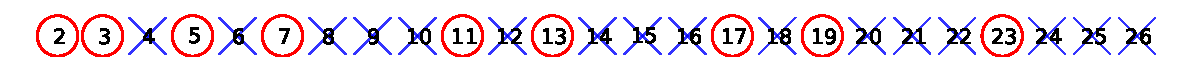
\includegraphics[width=\textwidth]{illustrations/circled_primes}
\end{frame}

\begin{frame}\frametitle{\bf The uiquity of primes}
\ill{dulcinea1}{.2}{Don Quixote and ``his'' Dulcinea del Toboso}

Numbers are obstreperous things. Don Quixote encountered this when he
requested that the ``bachelor'' compose a poem to his lady Dulcinea del
Toboso, the first letters of each line spelling out her name. The
``bachelor'' found




\begin{quote}
  ``a great difficulty in their composition because the number of
  letters in her name was $17$, and if he made four Castilian stanzas
  of four octosyllabic lines each, there would be one letter too many,
  and if he made the stanzas of five octosyllabic lines each, the ones
  called {\em d{\'e}cimas} or {\em redondillas,} there would be three
  letters too few...'' \bibnote{See Chapter IV of the Second Part of the Ingenius Gentleman Don Quixote of La Mancha.}
\end{quote}

``It must fit in, however, you do it,'' pleaded Quixote, not willing to
grant the imperviousness of the number $17$ to division.
\end{frame}

\end{document}
%sagemathcloud={"zoom_width":90}